\begin{frame}{Post Hoc Tests}
    Another term for multiple comparisons is \textbf{post hoc tests} (analyses done after an ANOVA).
    \begin{itemize}
        \item For a factorial experiment, we have three possible sets of comparisons.
        \begin{enumerate}
            \item Means for factor A
            \item Means for factor B
            \item Means for the factor level combinations (relating to interaction)
        \end{enumerate}
    \end{itemize}
\end{frame}

\begin{frame}{Post Hoc Tests}
    \begin{itemize}
        \item For the previous example, we have factor level combinations
        \begin{enumerate}
            \item Supervisor 1 with Day Shift
            \item Supervisor 1 with Swing Shift
            \item Supervisor 1 with Night Shift
            \item Supervisor 2 with Day Shift
            \item Supervisor 2 with Swing Shift
            \item Supervisor 2 with Night Shift
        \end{enumerate}
        \item This results in $\frac{k(k-1)}{2}=\frac{6\times5}{2}=15$ possible pairs.
    \end{itemize}
\end{frame}

\begin{frame}{Revisiting Multiple Comparisons}
    While the Bonferroni correction is effective and a standard approach in many fields, it represents a "worse case scenario" approach.
    \begin{itemize}
        \item This means it can sometimes be too aggressive.
        \item Naturally, this may not always be ideal.
        \item We want other options!
    \end{itemize}
\end{frame}

\begin{frame}{Tukey's Honest Significant Difference}
    For Tukey's method for paired comparisons
    \begin{itemize}
        \item The Type I error will be $\alpha$.
        \item The ANOVA assumptions are necessary.
        \begin{itemize}
            \item But if we do these tests post-ANOVA, these are already satisfied.
        \end{itemize}
        \item In addition, we must have independent sample means and equal group sizes.
    \end{itemize}
\end{frame}

\begin{frame}{Tukey's Honest Significant Difference}
    We will compare a value $\omega$ to differences in population means.
    \begin{itemize}
        \item This represents the \textbf{honest significant difference}.
        \item If $|\bar{x}_i-\bar{x}_j| > \omega$, we conclude that $\mu_i$ is different from $\mu_j$.
    \end{itemize}
\end{frame}

\begin{frame}{Tukey's Honest Significant Difference}
    \[
        \omega = q_{\alpha}(k, df)\left(\frac{s}{\sqrt{n_t}}\right)
    \]
    where
    \begin{itemize}
        \item $k=$ number of treatments (factor level combinations)
        \item $s^2=$ MSE, the estimate of the common variance $\sigma^2$
        \item $df=$ degrees of freedom for $s^2=$MSE
        \item $n_t=$ the number of observations in each treatment
        \item $q_{\alpha}(k, df)$ comes from Tukey's table of critical values
    \end{itemize}
\end{frame}

\begin{frame}{Example}
    Suppose you want to make pairwise comparisons for an ANOVA
    \begin{itemize}
        \item $k =5$ means 
        \item $\alpha=0.05$
        \item $s^2$ has 9 $df$
    \end{itemize}
\end{frame}

\begin{frame}{Tukey's Table of Critical Values}
    \begin{figure}
        \centering
        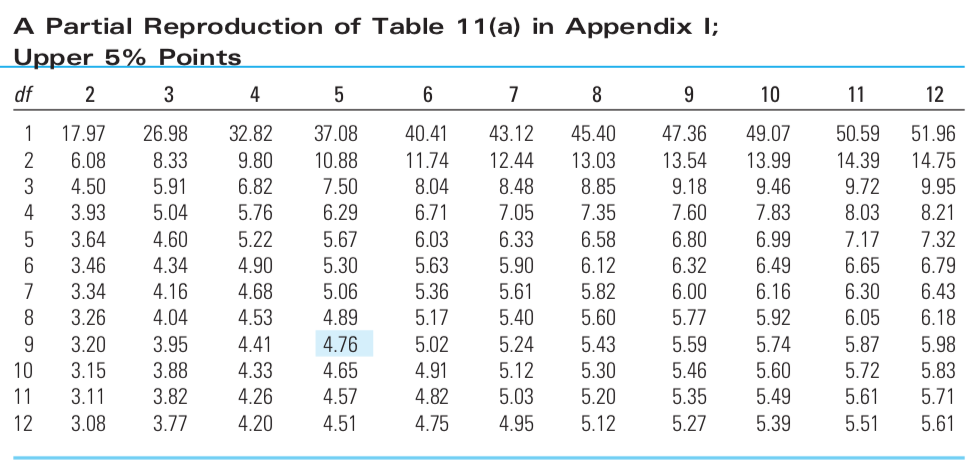
\includegraphics[width=\textwidth]{images/tukeycvs.png}
    \end{figure}
\end{frame}

\begin{frame}{Example}
    We have an experiment to determine the effect of nutrition on attention span of elementary school students.
    \begin{itemize}
        \item 15 students were randomly assigned to each of three meal plans:
        \begin{itemize}
            \item no breakfast
            \item light breakfast
            \item full breakfast
        \end{itemize}
        \item Attention spans were recorded during a morning reading.
    \end{itemize}
\end{frame}

\begin{frame}[fragile]{Example}
    The ANOVA table for this experiment (from \texttt{R}) is:
    \begin{verbatim}
        > summary(aov(span~trt))
                    Df Sum Sq Mean Sq F value Pr(>F)  
        trt          2  58.53  29.267   4.933 0.0273 *
        Residuals   12  71.20   5.933                 
    \end{verbatim}
    What can we conclude?
\end{frame}

\begin{frame}{Example}
    Calculate Tukey's yardstick for this ANOVA.
\end{frame}

\begin{frame}{Tukey's Table of Critical Values}
    \begin{figure}
        \centering
        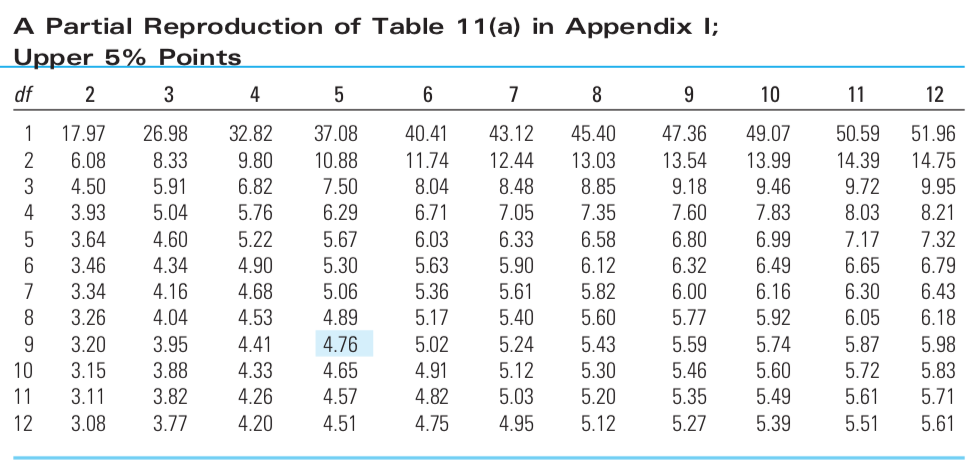
\includegraphics[width=\textwidth]{images/tukeycvs.png}
    \end{figure}
\end{frame}

\begin{frame}{Example}
    \begin{table}[h]
        \centering
        \begin{tabular}{lccc}
            \hline
            Treatment       & Mean & Standard Deviation \\
            \hline
            No Breakfast    & 9.4 & 2.30 \\
            Light Breakfast & 14 & 2.55 \\
            Full Breakfast  & 13 & 2.50 \\
            \hline
        \end{tabular}
    \end{table}
\end{frame}

\begin{frame}[fragile]{Tukey's Method in R}
    \begin{verbatim}
        > TukeyHSD(aov(span~trt))
          Tukey multiple comparisons of means
            95% family-wise confidence level

        Fit: aov(formula = span ~ trt)

        $trt
                    diff      lwr        upr     p adj
        light-full  1.0 -3.110011  5.1100111 0.7963670
        none-full  -3.6 -7.710011  0.5100111 0.0886624
        none-light -4.6 -8.710011 -0.4899889 0.0284289
    \end{verbatim}
\end{frame}

\begin{frame}{Example: Tukey's Method for More Complex ANOVAs}
    We will bring our example back to the supervisor and shift problem.
    \begin{itemize}
        \item We know there is a difference between the two supervisors.
        \item We will use Tukey's approach to compare each treatment (factor level combination).
    \end{itemize}
\end{frame}

\begin{frame}{Example}
    The ANOVA we found last class was
    \begin{table}[h]
        \centering
        \begin{tabular}{lcccc}
            \hline
            Source & $df$ & SS & MS & F \\ 
            \hline
            Supervisor (A)   & 1 & 19208 & 19208 & 26.68 \\
            Shift (B)        & 2 & 247   & 123.5 & 0.17 \\
            Interaction (AB) & 2 & 81127 & 40563.5 & 56.34 \\
            Error            & 12 & 8640 & 720 & \\
            Total            & 17 & 109222 & & \\
            \hline
        \end{tabular}
    \end{table}
\end{frame}

\begin{frame}{Example}
    Our treatment means looked like 
    \begin{table}[h]
        \centering
        \begin{tabular}{lccc}
             & \multicolumn{3}{c}{Shift} \\
            \cline{2-4}
            Supervisor & Day & Swing & Night \\
            \hline
            1 & 602 & 498 & 450 \\
            2 & 487 & 602 & 657 \\
            \hline
        \end{tabular}
    \end{table}
    There are $k=6$ treatments.
\end{frame}

\begin{frame}[fragile]{Example}
    \begin{verbatim}
            s2night s1day s2swing s1swing s2day s1night
    s2night       -    55      55     159   170     207
    s1day         -     -       0     104   115     152
    s2swing       -     -       -     104   115     152
    s1swing       -     -       -       -    11      48
    s2day         -     -       -       -     -      37
    s1night       -     -       -       -     -       -
    \end{verbatim}
\end{frame}
